According to the operation principle, WPT systems can be categorized as \textit{maximum power transfer} that maximizes the coverage and \textit{maximum energy efficiency transfer} that compromise with the power budget \cite{Hui2014}. Fig. \ref{fig:wpt-block-diagram} illustrates the fundamental blocks of a generic far-field WPT system.

\begin{figure}[ht]
  \centering
    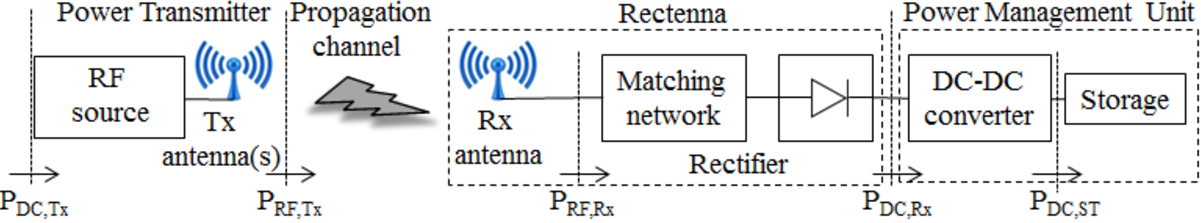
\includegraphics[width=\textwidth]{wpt_block_diagram}
  \caption{Block diagram of a generic far-field WPT system \cite{Clerckx2018a}}
  \label{fig:wpt-block-diagram}
\end{figure}

The transmit power efficiency $e$ is decomposed as

\begin{equation}\label{eqn:power_utilization_efficiency}
  e = \frac{{{P_{{\text{dc}},{\text{ST}}}}}}{{P_{{\text{dc}}}^t}} = \underbrace {\frac{{P_{{\text{rf}}}^t}}{{P_{{\text{dc}}}^t}}}_{{e_1}} \cdot \underbrace {\frac{{P_{{\text{rf}}}^r}}{{P_{{\text{rf}}}^t}}}_{{e_2}} \cdot \underbrace {\frac{{P_{{\text{dc}}}^r}}{{P_{{\text{rf}}}^r}}}_{{e_3}} \cdot \underbrace {\frac{{{P_{{\text{dc}},{\text{ST}}}}}}{{P_{{\text{dc}}}^r}}}_{{e_4}}
\end{equation}

Most existing solutions assumed no dependency among the components and focused on maximizing each term individually. Nevertheless, it has been proved by \cite{Boshkovska2015, Clerckx2016, Zeng2017} that these efficiencies are indeed coupled with each other, especially when input power is not very high (below \SI{1}{\mW}). Specifically, the DC-to-RF efficiency ${e_1}$ is related to signal PAPR and waveform design \cite{Boaventura2011}. Similarly, the RF-to-RF efficiency ${e_2}$ is determined by the channel state and the signal characteristics as waveform, beamformer, modulation, and power allocation \cite{Clerckx2019}. It also desires a highly directional transmission \cite{Takahashi2011}. ${e_3}$ measures the RF-to-DC efficiency of the rectenna, which is a function of input power ${P_{{\text{rf}}}^r}$ \cite{Trotter2009, Chen2017, Clerckx2018a}, channel state \cite{Clerckx2016, Clerckx2018}, and the waveform design \cite{Collado2014, Boaventura2015, Clerckx2019}. The DC-to-DC efficiency ${e_4}$ can be improved by dynamically adjusting the load of the rectifier according to the diode impedance \cite{Dolgov2010}.

Therefore, waveform design plays an essential role in WPT systems by contributing to ${e_1}, {e_2}, {e_3}$ simultaneously. To maximize the overall power efficiency $e$, we establish an tractable relationship between the transmitted signal and the harvester output current in the following section.